\documentclass[tikz,border=10pt]{standalone}
\usepackage{tikz}

\begin{document}
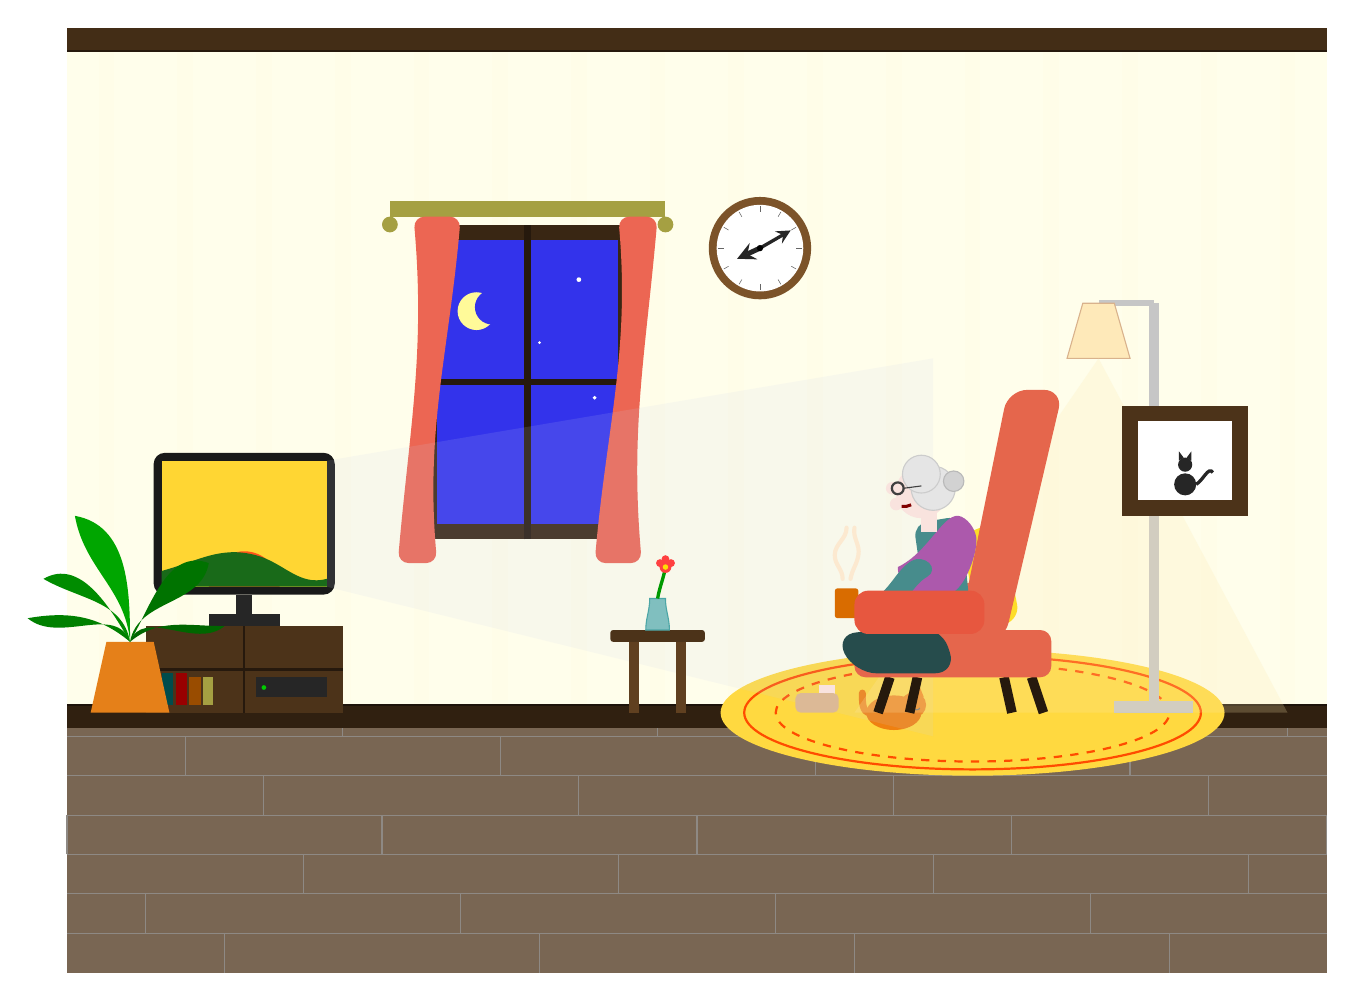
\begin{tikzpicture}[x=1cm, y=1cm]

% Background Wall (Warm cozy cream/peach color)
\fill[fill=orange!12!yellow!8!white] (0,3.3) rectangle (16,12.0);

% Wallpaper texture lines (Soft subtle vertical panels)
\foreach \x in {0.5,1.5,...,15.5} {
    \fill[orange!18!yellow!10!white, opacity=0.4] (\x,3.3) ++(-0.1,0) rectangle ++(0.2,8.4);
}

% Ceiling Molding
\fill[brown!35!black] (0,11.7) rectangle (16,12.0);
\draw[brown!20!black, thick] (0,11.7) -- (16,11.7);

% Wood Floor
\fill[fill=brown!40!black!75] (0,0) rectangle (16,3.3);

% Floor planks lines
\foreach \y in {0.5, 1.0, 1.5, 2.0, 2.5, 3.0} {
    \draw[brown!15!black!50, thin] (0,\y) -- (16,\y);
}

% Floor planks joints (vertical lines for realism)
\foreach \x in {2, 6, 10, 14} { \draw[brown!15!black!50, thin] (\x, 0) -- (\x, 0.5); }
\foreach \x in {1, 5, 9, 13} { \draw[brown!15!black!50, thin] (\x, 0.5) -- (\x, 1.0); }
\foreach \x in {3, 7, 11, 15} { \draw[brown!15!black!50, thin] (\x, 1.0) -- (\x, 1.5); }
\foreach \x in {0, 4, 8, 12, 16} { \draw[brown!15!black!50, thin] (\x, 1.5) -- (\x, 2.0); }
\foreach \x in {2.5, 6.5, 10.5, 14.5} { \draw[brown!15!black!50, thin] (\x, 2.0) -- (\x, 2.5); }
\foreach \x in {1.5, 5.5, 9.5, 13.5} { \draw[brown!15!black!50, thin] (\x, 2.5) -- (\x, 3.0); }
\foreach \x in {3.5, 7.5, 11.5, 15.5} { \draw[brown!15!black!50, thin] (\x, 3.0) -- (\x, 3.3); }

% Baseboard
\fill[fill=brown!25!black] (0,3.1) rectangle (16,3.4);
\draw[brown!15!black, thick] (0,3.4) -- (16,3.4);

% Cozy Patterned Rug
\fill[orange!40!yellow!75] (11.5, 3.3) ellipse (3.2 and 0.8);
\draw[orange!60!red, thick] (11.5, 3.3) ellipse (2.9 and 0.72);
\draw[orange!60!red, dashed, thick] (11.5, 3.3) ellipse (2.5 and 0.62);

% Sleeping Cat on Rug (Extremely cozy element)
\fill[orange!75!brown] (10.5, 3.3) ellipse (0.35 and 0.22);
\fill[orange!75!brown] (10.75, 3.4) circle (0.16);
\fill[orange!85!brown] (10.68, 3.5) -- (10.72, 3.65) -- (10.78, 3.52) -- cycle;
\fill[orange!85!brown] (10.78, 3.52) -- (10.82, 3.65) -- (10.88, 3.5) -- cycle;
\draw[orange!75!brown, line width=2.5pt, cap=round] (10.2, 3.3) to[out=180,in=270] (10.1, 3.55);
\draw[black!60, thin] (10.75, 3.36) to[out=280,in=260] (10.83, 3.36);

% Window with Curtains
\fill[brown!30!black] (4.5, 5.5) rectangle (7.2, 9.5);
\fill[blue!90!black!80] (4.7, 5.7) rectangle (7.0, 9.3);
% Outside Night Scene: Crescent Moon and Stars
\fill[yellow!40!white] (5.2, 8.4) circle (0.24);
\fill[blue!90!black!80] (5.4, 8.45) circle (0.22); % Cut out moon shape
\fill[white] (6.5, 8.8) circle (0.03);
\fill[white] (6.0, 8.0) circle (0.02);
\fill[white] (6.7, 7.3) circle (0.025);
% Window Panes Grid
\draw[brown!20!black, line width=2.5pt] (4.5, 7.5) -- (7.2, 7.5);
\draw[brown!20!black, line width=2.5pt] (5.85, 5.5) -- (5.85, 9.5);
% Curtain Rod
\fill[yellow!60!black] (4.1, 9.6) rectangle (7.6, 9.8);
\fill[yellow!60!black] (4.1, 9.5) circle (0.1);
\fill[yellow!60!black] (7.6, 9.5) circle (0.1);
% Draped Curtains
\fill[red!60!brown!75, rounded corners=4pt] (4.2, 5.2) to[out=85,in=275] (4.4, 9.6) -- (5.0, 9.6) to[out=265,in=95] (4.7, 5.2) -- cycle;
\fill[red!60!brown!75, rounded corners=4pt] (6.7, 5.2) to[out=85,in=275] (7.0, 9.6) -- (7.5, 9.6) to[out=265,in=95] (7.3, 5.2) -- cycle;

% Wall Clock (Shows peaceful evening time ~8:10 PM)
\fill[brown!65!black] (8.8, 9.2) circle (0.65);
\fill[white] (8.8, 9.2) circle (0.55);
\foreach \a in {0, 30, ..., 330} {
    \draw[black!60, very thin] (8.8, 9.2) ++(\a:0.46) -- ++(\a:0.07);
}
\draw[black!85, line width=1.8pt, -stealth] (8.8, 9.2) -- ++(205:0.32); % Hour hand
\draw[black!85, line width=1.2pt, -stealth] (8.8, 9.2) -- ++(30:0.45);  % Minute hand
\fill[black] (8.8, 9.2) circle (0.04);

% TV Stand / Console
\fill[brown!40!black] (1.0, 3.3) rectangle (3.5, 4.4);
\draw[brown!20!black, thick] (1.0, 3.85) -- (3.5, 3.85);
\draw[brown!20!black, thick] (2.25, 3.3) -- (2.25, 4.4);
% Small details inside console shelves (books and DVD player)
\fill[teal!60!black] (1.2, 3.4) rectangle (1.35, 3.8);
\fill[red!60!black] (1.38, 3.4) rectangle (1.52, 3.8);
\fill[orange!60!black] (1.55, 3.4) rectangle (1.7, 3.75);
\fill[yellow!60!black] (1.73, 3.4) rectangle (1.85, 3.75);
\fill[black!85] (2.4, 3.5) rectangle (3.3, 3.75);
\fill[green!80!black] (2.5, 3.62) circle (0.03);

% TV Set
\fill[black!85] (1.8, 4.4) rectangle (2.7, 4.55); % Base
\fill[black!85] (2.15, 4.55) rectangle (2.35, 4.8); % Neck
\fill[black!90, rounded corners=4pt] (1.1, 4.8) rectangle (3.4, 6.6); % TV Frame
\fill[cyan!10!blue!90] (1.2, 4.9) rectangle (3.3, 6.5); % Glowy Screen
% Beautiful Sunset Landscape Displayed on TV Screen
\begin{scope}
    \clip (1.2, 4.9) rectangle (3.3, 6.5);
    \fill[orange!40!yellow!80] (1.2, 4.9) rectangle (3.3, 6.5);
    \fill[red!50!orange!90] (2.25, 4.9) circle (0.45); % Sunset Sun
    \fill[green!35!black!90] (1.2, 4.9) -- (1.2, 5.1) to[out=15,in=165] (2.4, 5.3) to[out=345,in=195] (3.3, 5.0) -- (3.3, 4.9) -- cycle;
\end{scope}

% TV Light Beam (Cyan soft projection towards Grandma)
\fill[cyan!40!blue!20, opacity=0.13] (3.3, 4.9) -- (11.0, 3.0) -- (11.0, 7.8) -- (3.3, 6.5) -- cycle;

% Coffee / Side Table
\draw[brown!50!black, line width=3.5pt] (7.2, 3.3) -- (7.2, 4.2);
\draw[brown!50!black, line width=3.5pt] (7.8, 3.3) -- (7.8, 4.2);
\fill[brown!40!black, rounded corners=1pt] (6.9, 4.2) rectangle (8.1, 4.35);
% Red flower vase on the table
\fill[teal!50!white, draw=teal!70] (7.35, 4.35) to[out=90,in=270] (7.4, 4.75) -- (7.6, 4.75) to[out=270,in=90] (7.65, 4.35) -- cycle;
\draw[green!60!black, line width=1.2pt] (7.5, 4.75) to[out=80,in=260] (7.6, 5.15);
\fill[red!75!white] (7.6, 5.15) circle (0.075);
\fill[red!75!white] (7.53, 5.2) circle (0.05);
\fill[red!75!white] (7.67, 5.2) circle (0.05);
\fill[red!75!white] (7.6, 5.25) circle (0.05);
\fill[yellow!80!orange] (7.6, 5.15) circle (0.035);

% Cozy Floor Lamp (Casting warm yellow glow)
\fill[gray!45] (13.3, 3.3) rectangle (14.3, 3.45);
\draw[gray!45, line width=3.5pt] (13.8, 3.45) -- (13.8, 8.5);
\draw[gray!45, line width=2pt] (13.8, 8.5) -- (13.1, 8.5);
\fill[yellow!40!orange!25, draw=brown!60] (12.7, 7.8) -- (13.5, 7.8) -- (13.3, 8.5) -- (12.9, 8.5) -- cycle;
% Floor Lamp Light Cone (Soft warm ambient light)
\fill[yellow!50!orange!30, opacity=0.22] (13.1, 7.8) -- (10.0, 3.3) -- (15.5, 3.3) -- (13.1, 7.8) -- cycle;

% Comfortable Armchair (Soft warm colors)
% Legs
\draw[brown!20!black, line width=3.5pt] (10.3, 3.3) -- (10.45, 3.75);
\draw[brown!20!black, line width=3.5pt] (10.7, 3.3) -- (10.8, 3.75);
\draw[brown!20!black, line width=3.5pt] (12.0, 3.3) -- (11.9, 3.75);
\draw[brown!20!black, line width=3.5pt] (12.4, 3.3) -- (12.25, 3.75);
% Armrest (Far side)
\fill[red!45!brown!75, rounded corners=5pt] (10.4, 4.4) rectangle (11.8, 4.95);
% Yellow Pillow/Cushion behind back
\fill[yellow!75!orange!85, rounded corners=5pt] (11.6, 4.3) -- (12.1, 4.5) -- (11.85, 5.75) -- (11.35, 5.55) -- cycle;
% Armchair Cushion
\fill[red!50!brown!80, rounded corners=4pt] (10.0, 3.75) rectangle (12.5, 4.35);
% Tall Backrest
\fill[red!50!brown!80, rounded corners=7pt] (11.9, 4.2) -- (12.65, 7.4) -- (11.95, 7.4) -- (11.3, 4.2) -- cycle;

% Grandma (Lonely sweet grandma looking at the TV)
% Long teal/green skirt
\fill[teal!35!black!85, rounded corners=8pt] (10.0, 3.8) -- (11.3, 3.8) -- (11.1, 4.4) -- (9.75, 4.3) -- cycle;
% Feet and slippers
\fill[pink!75!brown!35] (9.55, 3.45) rectangle (9.75, 3.65);
\fill[brown!55!white, rounded corners=2pt] (9.25, 3.3) rectangle (9.8, 3.55);

% Torso
\fill[teal!60!gray!90, rounded corners=5pt] (10.95, 4.3) -- (11.5, 4.3) -- (11.35, 5.8) -- (10.75, 5.7) -- cycle;
% Warm knitted shawl draped over shoulders
\fill[violet!65!white, rounded corners=6pt] (10.55, 5.15) to[out=25,in=155] (11.55, 5.7) to[out=270,in=0] (10.95, 4.8) to[out=180,in=270] (10.55, 5.15);

% Head & Neck
\fill[pink!75!brown!35] (10.85, 5.6) rectangle (11.05, 5.9); % Neck
\fill[pink!75!brown!35] (10.85, 6.1) circle (0.33);          % Face
% Profile Details (Eye/Glasses level, gentle chin and small nose facing left)
\fill[pink!75!brown!35] (10.53, 5.95) circle (0.08);          % Chin
\fill[pink!75!brown!35] (10.48, 6.15) circle (0.08);          % Nose
\fill[pink!75!brown!35] (10.6, 6.0) rectangle (10.9, 6.2);    % Face bridge
% Gentle, peaceful smile
\draw[red!50!black, line width=1.1pt] (10.6, 5.92) to[out=350,in=200] (10.72, 5.94);

% Classic Bun Hair (White/Gray hair)
\fill[gray!20!white, draw=gray!40] (11.0, 6.15) circle (0.28);  % Back hair
\fill[gray!20!white, draw=gray!40] (10.85, 6.33) circle (0.24); % Top hair
\fill[gray!35!white, draw=gray!55] (11.26, 6.24) circle (0.13); % Hair Bun

% Reading Glasses
\draw[black!75, line width=0.8pt] (10.55, 6.15) circle (0.075);
\draw[black!75, thin] (10.62, 6.15) -- (10.85, 6.18);

% Arms holding a warm mug (Gazing and drinking tea)
\fill[teal!60!gray!90, rounded corners=4pt] (10.85, 5.3) to[out=210,in=30] (10.15, 4.7) -- (10.35, 4.5) to[out=30,in=210] (11.05, 5.1) -- cycle;
\fill[pink!75!brown!35] (10.1, 4.65) circle (0.075);
% Orange Tea Mug
\fill[orange!85!black, rounded corners=1pt] (9.75, 4.5) rectangle (10.05, 4.88);
\draw[orange!85!black, line width=1.5pt] (10.05, 4.69) circle (0.075);
% Steam curls rising from the hot tea
\draw[orange!25!white, line width=1.5pt, opacity=0.6, cap=round] (9.85, 5.0) to[out=90,in=270] (9.75, 5.3) to[out=90,in=270] (9.9, 5.65);
\draw[orange!25!white, line width=1.5pt, opacity=0.6, cap=round] (9.95, 5.0) to[out=80,in=260] (10.05, 5.3) to[out=80,in=260] (10.0, 5.65);

% Near Armrest (Covers part of body line for correct 3D perspective)
\fill[red!55!brown!85, rounded corners=5pt] (10.0, 4.3) rectangle (11.65, 4.85);

% Large Potted Monstera Plant in corner (Brings life and domestic feel to space)
\fill[orange!60!brown] (0.3, 3.3) -- (0.5, 4.2) -- (1.1, 4.2) -- (1.3, 3.3) -- cycle;
\fill[green!55!black] (0.8, 4.2) to[out=120,in=30] (-0.3, 5.0) to[out=330,in=100] (0.8, 4.2);
\fill[green!45!black] (0.8, 4.2) to[out=60,in=160] (1.8, 5.2) to[out=260,in=80] (0.8, 4.2);
\fill[green!65!black] (0.8, 4.2) to[out=90,in=350] (0.1, 5.8) to[out=280,in=95] (0.8, 4.2);
\fill[green!50!black] (0.8, 4.2) to[out=140,in=10] (-0.5, 4.5) to[out=320,in=110] (0.8, 4.2);
\fill[green!40!black] (0.8, 4.2) to[out=40,in=180] (2.0, 4.4) to[out=220,in=70] (0.8, 4.2);

% Family Picture Frame on the wall (A heartwarming touch of a cat painting)
\fill[brown!40!black] (13.4, 5.8) rectangle (15.0, 7.2);
\fill[white] (13.6, 6.0) rectangle (14.8, 7.0);
\fill[black!85] (14.2, 6.2) circle (0.14); % Cat body
\fill[black!85] (14.2, 6.45) circle (0.09); % Cat head
\fill[black!85] (14.12, 6.5) -- (14.12, 6.62) -- (14.18, 6.54) -- cycle; % Left ear
\fill[black!85] (14.28, 6.5) -- (14.28, 6.62) -- (14.22, 6.54) -- cycle; % Right ear
\draw[black!85, line width=1.2pt] (14.34, 6.2) to[out=30,in=120] (14.55, 6.35); % Tail

\end{tikzpicture}
\end{document}
